
\documentclass[10pt,conference,a4paper,onecolumn]{article}%{IEEEtran} % altura de letra=10, conferencia, formato a4. "`argencon"' o "`IEEEtran"' es la clase del monumento, que si no es el estandar, tiene sus propias opciones, como "`conference"'.journal
\usepackage[lmargin=2.5cm,rmargin=1.5cm,top=1.5cm,bottom=1.5cm]{geometry} % es para acomodar los margenes

% Para comentar un codigo rapido es con ctrl+q y para descomendar es con ctrl+w
%\newcommand{\CLASSINPUTbottomtextmargin}{10mm} % redefino el margen inferior
%\usepackage[latin1]{inputenc} %acentos sin codigo extra
%\usepackage[cp1252]{inputenc}% utf8
\usepackage[utf8]{inputenc} %acentos sin codigo extra \usepackage[utf8]{inputenc}
\usepackage[compress]{cite} %Es para agregar la bibliografia al final
\usepackage{url} % para poner URL 
%\usepackage[pdftex]{graphicx} % PDFLaTeX
%\usepackage[dvipdfmx]{graphicx} % PDFLaTeX

%\usepackage[dvips]{graphicx} % LaTeX
%\DeclareGraphicsExtensions{.eps}

\usepackage{graphicx}%es para agregar imagenes
\usepackage{subfigure}  %es para las subfiguras
%\DeclareGraphicsExtensions{.eps,.png}
%\DeclareGraphicsExtensions{.png,.eps}
%\usepackage[spanish]{babel} % es para castellanizar algunos comandos
%\usepackage[spanish, es-tabla]{babel} % para que en vez de cuadro diga tabla
\usepackage[spanish,es-noshorthands,es-tabla]{babel} %agrega unos caracteres extra al spanish de babel
\usepackage{alltt} %Ver para que es esto, me parece que simplifica el "` vervatim"'
\usepackage{listings} % es para poder cargar los codigos y que se vean bonitos
%\usepackage{eps}  
\usepackage{chngcntr} % para los pies de pagina
\usepackage[hidelinks]{hyperref} % para agregar links "`[hidelinks]"' sirve para sacar el recuadro alrededor del link
\usepackage{amsthm} % ambiente matematico
\usepackage{amsmath} %otro ambiente matematico
%\usepackage{slashbox} % Es para poner la linea en la tabla
\usepackage[compress]{cite} %Es para agregar la bibliografia al final
%\usepackage{hyperref} % para poner un indice con que linkee a todo el texto en el pdf
\usepackage{color} % para poner textos con color 
\usepackage{hyperref} % para poner links
\usepackage{epsfig} % para poner color en las tablas
\usepackage{multirow}% para poner color en las tablas
\usepackage{colortbl}% para poner color en las tablas. Esta es la mas importante 
%\columncolor[Modelo]{Color}[SepIzq][SepDer] (columnas) \rowcolor[Modelo]{Color}[SepIzq][SepDer] (filas) 
% http://metodos.fam.cie.uva.es/~latex/apuntes/apuntes10.pdf
\usepackage[table]{xcolor}% para poner color en las tablas % http://ctan.org/pkg/xcolor
% ------------------- \newcommand
%\renewcommand{\tablename}{Tabla} % para que diga tabla en vez de ``cuadro''
\newcommand{\be}{\begin{equation}}  %Simplifica la escritura de ecuaciones
\newcommand{\ee}{\end{equation}}  %Simplifica la escritura de ecuaciones
\newcommand{\nbe}{\begin{equation*}}  %Simplifica la escritura de ecuaciones
\newcommand{\nee}{\end{equation*}}  %Simplifica la escritura de ecuaciones
\newcommand{\m}{\begin{bmatrix}}
\newcommand{\fm}{\end{bmatrix}}
\newcommand{\fig}[4]{ % Figuras asi se usa: \fig{Nombrefigura}{epigrafe}{donde? h, t, b, htb}{ancho}
\begin{figure}[#3]
\centering
\includegraphics[width=#4\columnwidth]{./Figuras/#1}
\caption{#2}\label{fig:#1}
\end{figure}}

\newcommand{\arr}[2]{ % es para poder apilar ecuaciones NO numeradas
\begin{equation*}
\begin{array}{#1} #2 
\end{array}
\end{equation*}}

\newcommand{\pap}{paso a paso\  }
\newcommand{\Mic}{microstepping}
\newcommand{\xx}{\cellcolor{blue!50}}

% --------------- FIN \newcommand ----------------------




\begin{document} % comienza el documento, es como el main.

%\title{Informe del Trabajo/Proyecto Final \\
%Accionamiento eléctrico para un motor paso a paso unipolar de reluctancia
%variable} % (?)


%\vspace{1cm} % Doy un espacio de 1cm de altura entre el titulo y el autor
\begin{titlepage}
\centering
\begin{Huge}
 
\textbf{Instituto Tecnológico del Comahue}  \\

\end{Huge}


\vspace{2cm}
\begin{figure}[h]
\centering
\includegraphics[width=3cm]{../Figuras/logoITC}
\end{figure}

\vspace{2cm}
\normalsize
\begin{LARGE}


 Computadoras Electrónicas \\

$6^{to}$ B  
 
 \end{LARGE}
 \vspace{2cm}
\begin{Large}
Guia de Trabajo Práctico de Laboratorio PWM, Conversión Analógica, Comunicaciones 
\end{Large}
\vspace{2cm}
\normalsize 
\begin{flushleft}
%Docente: Sansoni Sebastián 
Versión: 2.0 (\textbf{Beta})
\end{flushleft}

\vspace{1cm}


\centering Neuquén, \the\year \\


\vspace{1cm}



\end{titlepage}
  % \mbox es para que no corte la oracion 
%\author{Sansoni Sebastián \\
%\emph{Maquinas Eléctricas, Ingeniería Electrónica}\\ \emph{Docentes a cargo:  Ing. Labriola Carlos, Ing. Ávila Marcelo}\\ \emph{Año 2017} \\
%\emph{ Departamento de Electrotecnia, Facultad de ingeniería, Universidad Nacional del Comahue }\\ \emph{Buenos Aires 1400, Neuquén Capital, Argentina}\\ \emph{\small{\texttt{sansoni.sebas@gmail.com}}}} 

%\author{\IEEEauthorblockN{Sansoni Sebastián} %\vspace{0.2cm}
%\IEEEauthorblockA{\emph{Maquinas Eléctricas, Ingeniería Electrónica}\\ \emph{Docentes a cargo:  Ing. Labriola Carlos, Ing. Ávila Marcelo}\\ \emph{Año 2017} \\
%\emph{ Departamento de Electrotecnia, Facultad de ingeniería, Universidad Nacional del Comahue }\\ \emph{Buenos Aires 1400, Neuquén Capital, Argentina}\\ \emph{\small{\texttt{sansoni.sebas@gmail.com}}}}} 

% en este entorno, ademas del nombre del autor se agregan mas caracteristicas en el titulo, por eso estan los "`bloques del autor"'. "`\IEEEauthorblockN"' pone los nombres. "`\IEEEauthorblockA{}"' las Afiliaciones (todo lo demas).\\ agrega un enter
%\maketitle % Dice donde poner el \emph{titulo}

%\newpage % comenzar una nueva pagina 

%\tableofcontents

%\newpage

%\begin{abstract}

%\end{abstract}
%\begin{IEEEkeywords}Actitud, acelerómetro, estimación, seguimiento\end{IEEEkeywords}
\section{Objetivos}
El objetivo principal de estos ejercicios es incentivar la curiosidad del estudiante en los temas de este trabajo.\\
Como objetivos secundarios se establecen los siguientes:
\begin{itemize}
\item Familiarizarse con la conversión Digital - Analógica por medio de señales PWM. 
\item Apropiarse de los conocimientos relacionados con: Resolución, selección de frecuencia de un PWM, configuración de los módulos asociados con los timers.  
\item Obtener una primer aproximación hacia la conversión Analógica - Digital.
\item Apropiarse de los conocimientos relacionados con: Tensión de referencia, Impedancia de entrada del conversor, Tiempo de muestreo y Tiempos de conversión. 
\item Diferenciar las aplicaciones de los distintos protocolos de comunicación. Marcando los puntos fuertes y débiles de cada uno según la situación.  
\end{itemize}
 
 \section{Aspectos generales}
 
	Cuando se pide un \textbf{registro} del ejercicio, hace referencia a que tome nota o saque fotos de lo que se esta viendo o realizando  
 
 %Cuando se pide realizar un ejercicio desde el IDE de MPLAB, siempre se debe comprobar el funcionamiento con el debugger, salvo que se especifique lo contrario.
 
 %Cuando se pide realizar un ejercicio desde el IDE de Arduino, siempre se debe comprobar el funcionamiento programando el microcontrolador.

\section{PWM}
\subsection{IDE Arduino - Atmega328p}
\begin{enumerate}
\item \label{primero} Utilizando la función \emph{analogWrite()} de Arduino varié la intensidad de un led conectado en el pin $N^o 6 $   de manera que describa un diente de cierra con un periodo de 10 segundos. 
\item Realice el ejercicio \ref{primero} mismo ejercicio anterior solo que en vez de variar la intensidad del LED\_ BUILTIN se varié la de un  \emph{led externo} a la placa.
\item Utilizando un Osciloscopio \textbf{registre} la forma de onda de salida. Mida la \emph{frecuencia} de la señal.  
\item Diseñe un filtro pasa bajo de primer orden con frecuencia de corte $W_c \approx 1Hz$. En caso de no tener los componentes necesarios hágalo con $W_c < 1Hz$. Redacte de forma clara y concisa un documento explicando y justificando la selección de componentes, cálculos, etc. Puede apoyar el diseño con algún software de simulación como LTspice.
\item Conecte el filtro diseñado en el pin de la placa en donde estaba el led externo del 2do punto de esta sección. Por medio de un Osciloscopio  \textbf{registre} la \emph{tension} del capacitor.
\item Modifique el periodo de señal de diente de cierra a 0.5 segundos. \textbf{Registre} la \emph{tension} del capacitor. ¿Cual es la máxima frecuencia posible de esta señal tal que la salida tenga una amplitud de $4V$? Justifique.
\item Sin ayuda ajena al grupo de trabajo (compañeros, libros, internet, etc.) conjeture una explicación del porque cambio la forma de la señal de tension. 
\item Redacte un informe que contenga todos los registros y documentos  mencionados anteriormente, puede utilizar cualquier editor de texto. Debe ser entregado antes del \textbf{9/05/18} en formato PDF por medio de la plataforma chamilo. 

\item Identifique y haga un esquema de la placa Arduino que tenga, relevando cuales son los pines correspondientes a las salidas del modulo Compare. Tenga en cuenta que son 2 pines por cada Timer del -microcontrolador. Recomendación: ver la  tabla " \emph{Table 6-1 PORT Function Multiplexing} " de la pagina 16 del datasheet.
 \item Configure el \emph{Timer 2} en modo \textbf{Fast PWM} para que oscile a una frecuencia de \emph{$2kHz$}, que tenga un duty cycle de \emph{ $ 30 \% $ } y que salga por el pin \emph{OC2A}.
 \item Conecte al pin OC2A el filtro antes diseñado. Con ayuda de un Osciloscopio registre la tension del capacitor. ¿La tensión medida es constante en el tiempo?
 \item Calcule el  duty cycle para  obtener una tension de $ 3.3V $ en el capacitor. Respalde estos cálculos con datos medidos. 
\item  Calcule el  duty cycle para  obtener una tension de $ 3.14159V $ en el capacitor. ¿Cuál es la resolución de este generador de tensión?
 \item Configure el \emph{Timer 1} en modo \textbf{Fast PWM} para que oscile a una frecuencia de \emph{$10kHz$}, que tenga un duty cycle de \emph{ $ 45 \% $ } y que salga por el pin \emph{OC1A}.
 \item Conecte al pin OC1A el filtro antes diseñado. Mida la mínima \emph{variación} posible de tension sobre el capacitor. ¿Es mayor o menor comparada con la del timer 2? Justifique.

\end{enumerate}
 
\subsection{Problema de aplicación}
\begin{enumerate}
\item Utilizando los conocimientos previos y los generados en este trabajo, realice un generador de onda \emph{senoidal} de $100Hz$ y una amplitud $4V_{pp} $ 
 \item Redacte un informe que contenga todos los registros y documentos  mencionados anteriormente, puede utilizar cualquier editor de texto. Debe ser entregado antes del \textbf{16/05/18} en formato PDF por medio de la plataforma chamilo. 
\end{enumerate}

\section{ADC}
%Próximamente. \textbf{16/05/18 al 23/05/18}

\begin{enumerate}
\item  Por medio de la función analogRead() de arduino, lea una entrada analógica conectada a $V_{cc}$. Realice 10 mediciones espaciadas por 1 segundo. \textbf{Registre} el valor promedio de esas mediciones.\label{punto:Adc_1}
\item \label{punto:Adc_2} Rehaga el ejercicio \ref{punto:Adc_1} pero esta vez conectando la entrada analógica a GND.
\item \label{punto:Adc_3}  Realice un divisor resistivo con 2 resistencias iguales, conectándolas entre $V_{cc}$ y GND. Conecte el punto medio a una entrada analógica. Realice 10 mediciones espaciadas por 1 segundo. \textbf{Registre} el valor promedio de esas mediciones y  con ayuda de los valores obtenidos en los ejercicios \ref{punto:Adc_1} y \ref{punto:Adc_2} modele una función (matemática) tal que convierta los valores leídos a valores de tension. 
\item Por medio de otro divisor resistivo, obtenga en el punto medio una tension aproximada de $0.5V$. Por medio del osciloscopio \textbf{registre} el valor de tension obtenido. Luego conecte una entrada analógica a ese divisor resistivo. Utilice la función obtenida en el punto \ref{punto:Adc_3} para averiguar la tension medida. Calcule y \textbf{registre} el error de la medición considerando que el valor del osciloscopio es el valor real.   
\item Realice un divisor resistivo  con 2 resistencias de $100k\Omega$. Por medio de una entrada analógica y la función obtenida en el punto \ref{punto:Adc_3} \textbf{registre} la tensión medida. Mida la tension con un osciloscopio y compare los valores medidos con los esperados. Conjeture una explicación para lo sucedido. Observacion: se recomienda leer la pagina 312 del datasheet. (puede fallar)
\item Con ayuda de los registros elabore un informe. El mismo debe entregarse antes del \textbf{23/05/18}.
\end{enumerate}

\subsection{Problema de aplicacion}
Utilizando los conocimientos previos y los generados en este trabajo 
\begin{enumerate}
\item \label{punto:adc_PA1} Realice un circuito tal que lea una entrada analógica y que genere el mismo valor de tension por otro conector. 
\item Modifique el programa y el circuito implementado en el punto \ref{punto:adc_PA1} tal que sea capaz de de seguir una señal senoidal de $4V_{pp}$ de $33 Hz$. \textbf{Registre} la entrada y la salida generada con el microcontrolador.
\item Implemente el circuito de la figura \ref{fig:1}, considerando que la resistencia $R1$ es una LDR y $R3$ es del mismo valor que $R1$ cuando esta expuesta a la luz ambiente. \emph{PWM} hace referencia a una salida de PWM y \emph{ADC} a una entrada analógica.

\begin{figure}[h]
\centering
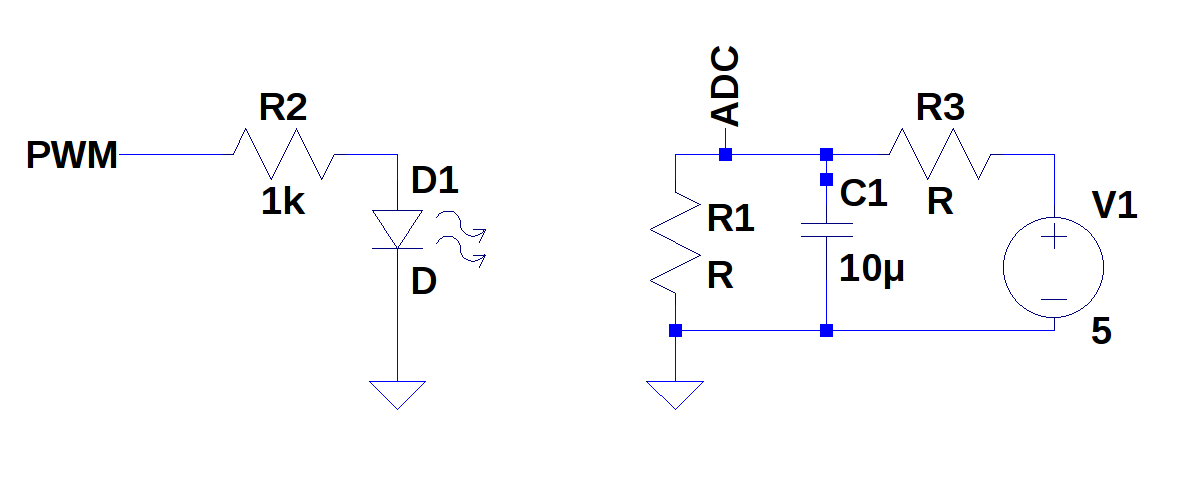
\includegraphics[width=10cm]{./imagenes/circuito_ldr.png}
\caption{Circuito propuesto para realizar un ejercicio de control.}
\label{fig:1}
\end{figure}

\item Realice un código tal que por medio del led $D1$ se pueda mantener una tension en $R1$ de $4.5V$. Se recomienda buscar información acerca de controladores proporcionales. 

\item Para acreditar esta parte se requiere mostrarle al profesor el trabajo funcionando. Preparar una breve exposición para demostrar los conocimientos adquiridos. Fecha limite de entrega \textbf{06/06/18}.
\end{enumerate}
\section{Comunicaciones}
Próximamente. \textbf{06/06/18 al 13/06/18} y \textbf{13/06/18 al 20/06/18}
%
%Hacer un trabajo corto para dar tiempo en hacer los otros tps. Ver el 2do cierre de trimestre. 
% En funcion de lo antes hecho establecer una comunicacion con varios nodos y generar algunas centrales.
%
%
\section{Problema de diseño}

\section{BIBLIOGRAFÍA ORIENTATIVA}

Paginas
\begin{itemize}
\item http://www.nongnu.org/avr-libc/
\item https://www.microchip.com/webdoc/AVRLibcReferenceManual/index.html
\item http://www.microchip.com/mplab/mplab-x-ide
\item https://garretlab.web.fc2.com/en/arduino/inside/index.html
\end{itemize}
%\nocite{*}  % Es para agregar toda la bibliografia de manera indiscriminada. 
\bibliographystyle{ieeetr}
%\nocite{PainaCareli}
%\nocite{nvidia2011nvidia}
%\nocite{bradski2008learning}
%\nocite{bishop2006pattern}
%\nocite{Stereolabs}
%\nocite{quigley2009ros}
%\nocite{jetson}
%\nocite{scaramuzza2011visual}
%\nocite{fraundorfer2012visual}


%\bibliography{biblioteca_plan}

%\begin{thebibliography}{X}
%\bibitem{Paina}Auat Cheein, F. A., Steiner, G., Perez Paina, G., \& Carelli, R. (2010). Aplicación de un EIF-SLAM en entornos agrícolas basado en detección de troncos de árboles.
%\bibitem{Farmers}Bergerman, M., Maeta, S. M., Zhang, J., Freitas, G. M., Hamner, B., Singh, S., \& Kantor, G. (2015). Robot farmers: Autonomous orchard vehicles help tree fruit production. IEEE Robotics \& Automation Magazine, 22(1), 54-63.
%
%%\bibitem{libros} Salazar, M.G. and Barahona, M.L. (2017). Methods in Engineering. Prentice Hall, Englewood Cliffs, NJ, USA.
%%\bibitem{revistas}Choleski,   R.L.   and   Kutta,   S.H.   (1982).   Reduced   noise and quadratic problem. Eng., v. 8, n. 3, p. 409-428.
%%\bibitem{congreso}Choleski,   R.L.   and   Kutta,   S.H.   (2002). Optimum design. Proceeding Electronic Congress, New York, May. % conferencias y seminarios
%%\bibitem{Tesis} Marcos,  A.  (2003). Evaluación de sistemas dinámicos.  Tesis doctoral, Universidad Nacional de Colombia. %o disertasiones
%%\bibitem{documento_tecnico} Marcos, A. (2004). Respuesta de modelos no lineales. Reporte Técnico Report B5875, Offshore Technology Research Center, USA.% o repores
%\end{thebibliography}




\end{document}
